% Just notes
%\documentclass[notes=only]{beamer}

% Both slides and notes
\documentclass[notes]{beamer}

% Just slides
% \documentclass{beamer}

\usetheme{default}

% Used to do math and such (I think...)
\usepackage{amsmath}
\usepackage{amssymb}

% Used to color text (for todos)
\usepackage{xcolor}

\usepackage{algorithm}
\usepackage{algpseudocode}

\usepackage{array}

% Used to embed pdfs from yEd and other sources
\usepackage{graphicx}

% Used to make code listings
\usepackage{listingsutf8}
% Used to adjust the page margin
\usepackage{geometry}
% Used to make code show up in multiple columns to fit more on a printed page.
\usepackage{multicol}

% Used to make tables, figures, etc show up where I want them.
\usepackage{float}

\usepackage{array}

%import figures from photoshop
\usepackage{epstopdf}

% Deal with backwards quotes because evidently Latex doesn't know better.
\usepackage [english]{babel}
\usepackage [autostyle, english = american]{csquotes}
\MakeOuterQuote{"}

% multiple rows
\usepackage{multirow}

% used for lettered bullet points
\usepackage{enumerate}

% http://tex.stackexchange.com/questions/137022/how-to-insert-page-number-in-beamer-navigation-bars
% Add page numbers
\addtobeamertemplate{navigation symbols}{}{%
    \usebeamerfont{footline}%
    \usebeamercolor[fg]{footline}%
    \hspace{1em}%
    \insertframenumber/\inserttotalframenumber
}

\usepackage{mathrsfs}

\newcommand{\TODO}[1]{\textcolor{red}{TODO: #1}}

\newcommand{\argmax}[1]{\underset{#1}{\text{argmax }}}
\newcommand{\cprob}[2]{ \prob{#1 \lvert #2} }
\newcommand{\prob}[1]{\mathbb{P}\left( #1 \right)}
\newcommand{\partialDx}[2]{\frac{\partial #1}{ \partial #2  }}
\newcommand{\inAngle}[1]{\left \langle #1 \right \rangle}


\begin{document}

\title{Deep Learning for Automatic Speech Recognition}
\subtitle{CSCI/LING-5832: Natural Language Processing}
\author{Ryan Hartsfield \and Garrett Lewellen}
\date{April 23, 2015}

\frame{\titlepage}

\begin{frame}
	\frametitle{Outline}
	
	\begin{enumerate}
		\item \textcolor{blue}{Introduction}
		\item Gaussian Mixture Models
		\item Convolutional Neural Networks
		\item Deep Neural Networks
		\item Experimental Results
		\item Conclusions
	\end{enumerate}
\end{frame}

\begin{frame}

\end{frame}

\begin{frame}

\end{frame}

\begin{frame}

\end{frame}

\begin{frame}

\end{frame}

\begin{frame}
	\frametitle{Outline}
	
	\begin{enumerate}
		\item Introduction
		\item \textcolor{blue}{Gaussian Mixture Models}
		\item Convolutional Neural Networks
		\item Deep Neural Networks
		\item Experimental Results
		\item Conclusions
	\end{enumerate}
\end{frame}

\begin{frame}

\end{frame}

\begin{frame}

\end{frame}

\begin{frame}

\end{frame}

\begin{frame}

\end{frame}

\begin{frame}
	\frametitle{Outline}
	
	\begin{enumerate}
		\item Introduction
		\item Gaussian Mixture Models
		\item \textcolor{blue}{Convolutional Neural Networks}
		\item Deep Neural Networks
		\item Experimental Results
		\item Conclusions
	\end{enumerate}
\end{frame}

\begin{frame}

\end{frame}

\begin{frame}

\end{frame}

\begin{frame}

\end{frame}

\begin{frame}

\end{frame}

\begin{frame}
	\frametitle{Outline}
	
	\begin{enumerate}
		\item Introduction
		\item Gaussian Mixture Models
		\item Convolutional Neural Networks
		\item \textcolor{blue}{Deep Neural Networks}
		\item Experimental Results
		\item Conclusions
	\end{enumerate}
\end{frame}

\begin{frame}{Deep Neural Networks}
	\begin{center}
	\textbf{Context-Dependent Pre-Trained Deep Neural Networks for Large-Vocabulary Speech Recognition}
	\end{center}
	
	\vfill

	\hfill George Dahl \hfill Dong Yi \hfill Li Deng \hfill Alex Acero \hfill
	
	\vfill
	
	\begin{center}
		IEEE Transactions on Audio, Speech, and Language processing, Vol. 20, No. 1, January 2012
	\end{center}
	
\end{frame}
	
\begin{frame}{Problem Formulation}
	\begin{center}
		Noisy channel model: maximize the likelihood of a decoded word sequence, $\hat{w}$, given our observed audio input, $x$:
	\end{center}
	 
	\vfill
	
	\begin{equation*}
		\hat{w} = \argmax{w \in \mathscr{L}} \underbrace{\cprob{x}{w}}_{\text{ Accoustic Model }} \underbrace{\prob{w}}_{\text{ Language Model }} 
	\end{equation*}
	
	\vfill
	
	\begin{center}
		Use N-gram language model, CD-DNN-HMM for acoustic model
	\end{center}
\end{frame}

\begin{frame}{Problem Formulation (Cont)}
	\begin{center}
	Here the acoustic model is viewed as a sequence of transitions between states of tied-state triphones referred to as \textbf{senones}.
	\end{center}
	
	\vfill
	
	\begin{equation*}
	\underbrace{\cprob{x}{w}}_{\text{ Accoustic Model }} \approxeq \max \underbrace{\pi(q_0)}_{ \text{ Init State } } \prod_{t = 1}^T \underbrace{ a_{q_{t-1} q_t} }_{ \text{ Transistion } } \prod_{t=0}^T \underbrace{ \cprob{x_t}{q_t} }_{ \text{ Senone posterior } } 
	\label{eqn:lm:def}
	\end{equation*}
	
	\vfill
	
	\begin{center}
		Where $\cprob{x_t}{q_t}$ models the tied triphone senone posterior given mel-frequency cepstral coefficients (\textbf{MFCCs}) based on 11 sampled frames of audio.
	\end{center}
\end{frame}
	
\begin{frame}{Deep Neural Networks}
	\resizebox{\linewidth}{!}{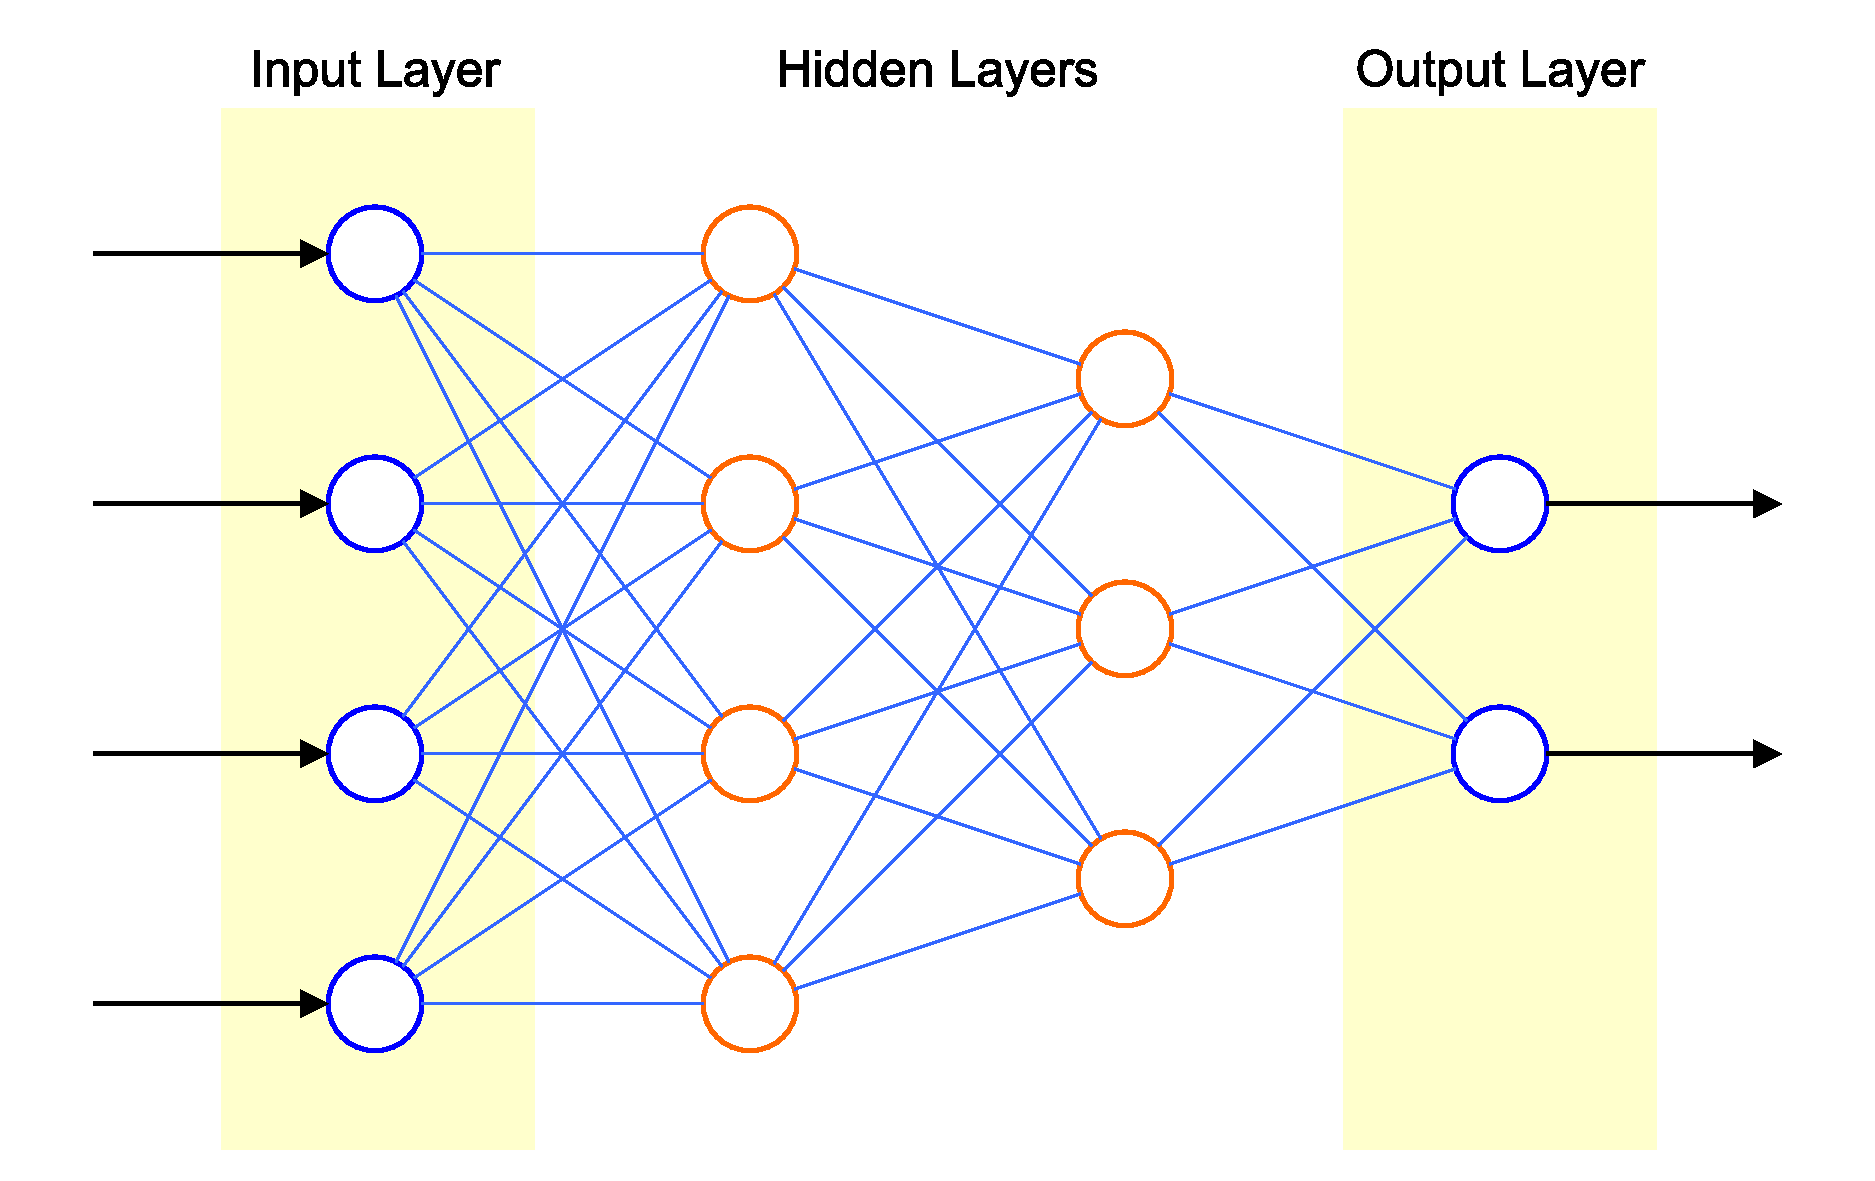
\includegraphics{dnn.pdf}}
\end{frame}

\begin{frame}{Training}
	\begin{center}
		Training is complicated and time intensive! At a very high level two steps: initialization and DNN training.
	\end{center}
	
	\vfill
	
	Initialization:
	\begin{itemize}
		\item Find the best tying of triphone states
		\item Deal with some book keeping
		\item Train a CD-GMM-HMM using those states.
		\item Convert CD-GMM-HMM into CD-DNN-HMM keeping senone structure
		\item Apply pre-training algorithm on CD-DNN-HMM
	\end{itemize}

	\vfill	

\end{frame}

\begin{frame}{Training}

\vfill

DNN Training:

\begin{itemize}
	\item Generate raw alignment of states to senones
	\item Use alignment to refine by backpropagation
	\item Re-estimate prior senone probability given frames
	\item Refine HMM transitions probabilities
	\item Goto first step if no improvement against development set
\end{itemize}

\vfill

\vfill

\begin{center}
Just enough time to talk about one of these steps in detail. Let's look at pre-training...
\end{center}

\vfill


\end{frame}


\begin{frame}{Pre-Training In-Depth}
	\vfill

	\begin{center}
		DNN training computationally intractable until Hinton et al. come to the rescue with \textit{A Fast Learning Algorithm for Deep Belief Nets}.
	\end{center}
	
	\vfill

	\begin{center}
		Big idea: Use an approximate method, \textbf{contrastive divergence}, to get near an optimal solution, then use traditional methods, \textbf{backpropagation}, to finish the job. 
	\end{center}
	
	\vfill
	
	\begin{center}
		Need to understand Restricted Boltzman Machines (RMBs) and Deep Belief Networks (DBNs)
	\end{center}
	
	\vfill
\end{frame}

\begin{frame}{Pre-Training: RBMs and DBNs}
	\vfill

	\begin{columns}
		\begin{column}{0.4\linewidth}
			\begin{center}
				Bipartite arrangement of weights is assigned an energy:
			\end{center}
		
			\begin{equation*}	
				E(v, h) = - b^T v - c^T h - v^T W h
			\end{equation*}
		\end{column}
		\begin{column}{0.6\linewidth}
			\resizebox{\linewidth}{!}{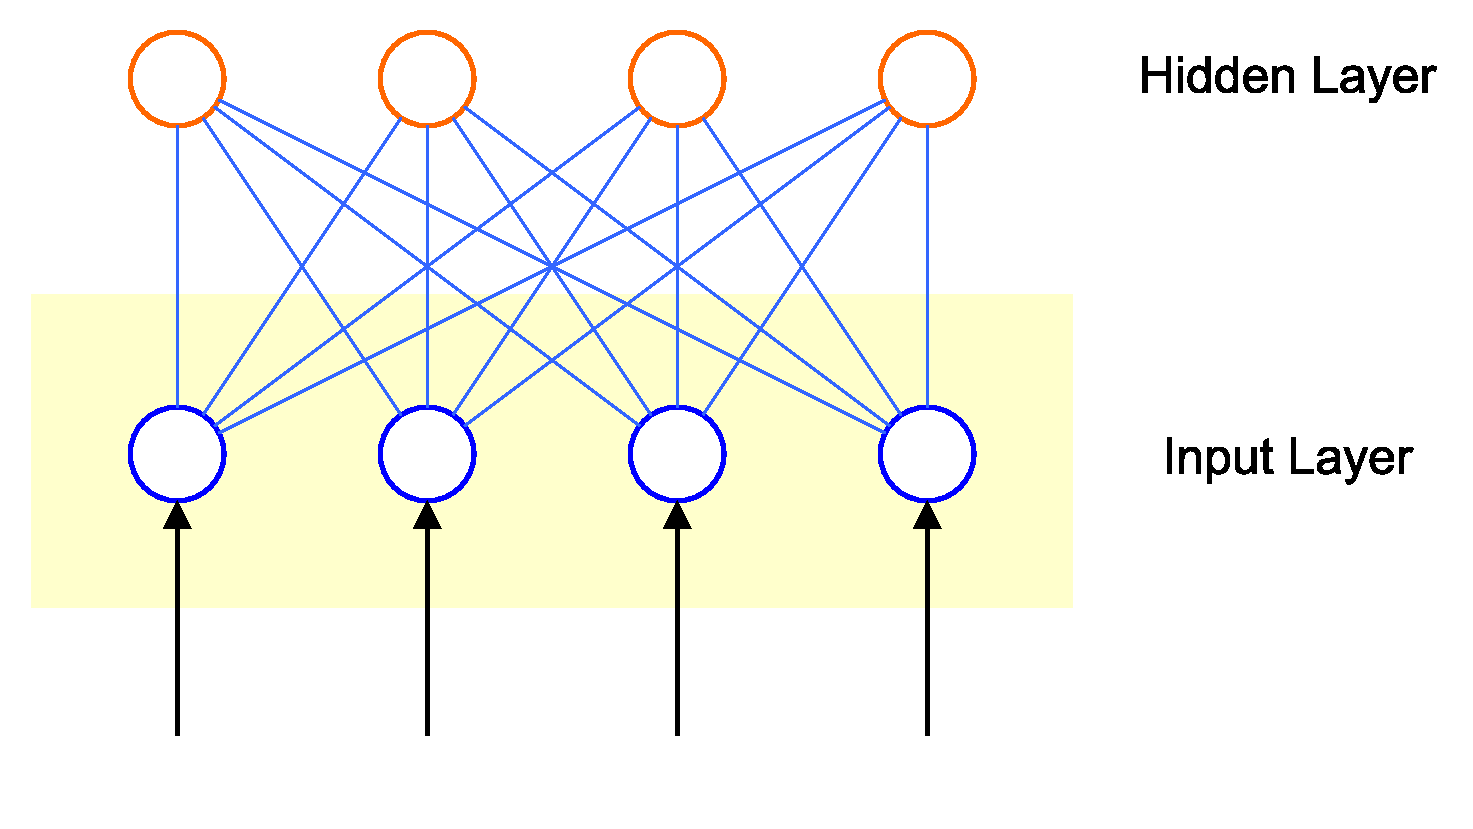
\includegraphics{rbm.pdf}}
		\end{column}
	\end{columns}
	
	\vfill

	\begin{center}
		For purpose of this talk, stack RBMs on top of one another to get a DBN
	\end{center}

	\vfill
\end{frame}

\begin{frame}{Pre-Training: Contrastive Divergence}
		\begin{center}
			Want to do vanilla Stochastic Gradient Descent, however, our \textcolor{blue}{model} term takes \textbf{exponential} time to compute correctly. 
		\end{center}
		
		\begin{equation*}
			- \partialDx{\ell(\theta)}{w_{ij}} = \inAngle{ \partialDx{E}{\theta} }_\text{data} - \inAngle{ \partialDx{E}{\theta} }_\text{\textcolor{blue}{model}}
		\end{equation*}
		
		\begin{center}
			Instead, \textbf{approximate} it (essentially minimizing Kullback-Leibler divergence) with \textcolor{blue}{one step} Gibbs sampling:
		\end{center}
		
		\begin{equation*}
			- \partialDx{\ell(\theta)}{w_{ij}} \approx \inAngle{ v_i h_j }_\text{data} - \inAngle{ v_i h_j }_\text{\textcolor{blue}{1}}
		\end{equation*}
\end{frame}

\begin{frame}{Pre-Training: Bringing it all together}
	\begin{columns}
		\begin{column}{0.45\linewidth}
			Hinton's Greedy Algorithm:
		
			\hfill
		
			1) Train RBM consisting of first two layers
			
			\hfill
			
			2) Move RBM frame up a layer and train

			\hfill 
			
			3) When out of layers, you have trained DBN
			
			\hfill
			
			4) Refine with backpropagation
		\end{column}
		\begin{column}{0.55\linewidth}
			\resizebox{\linewidth}{!}{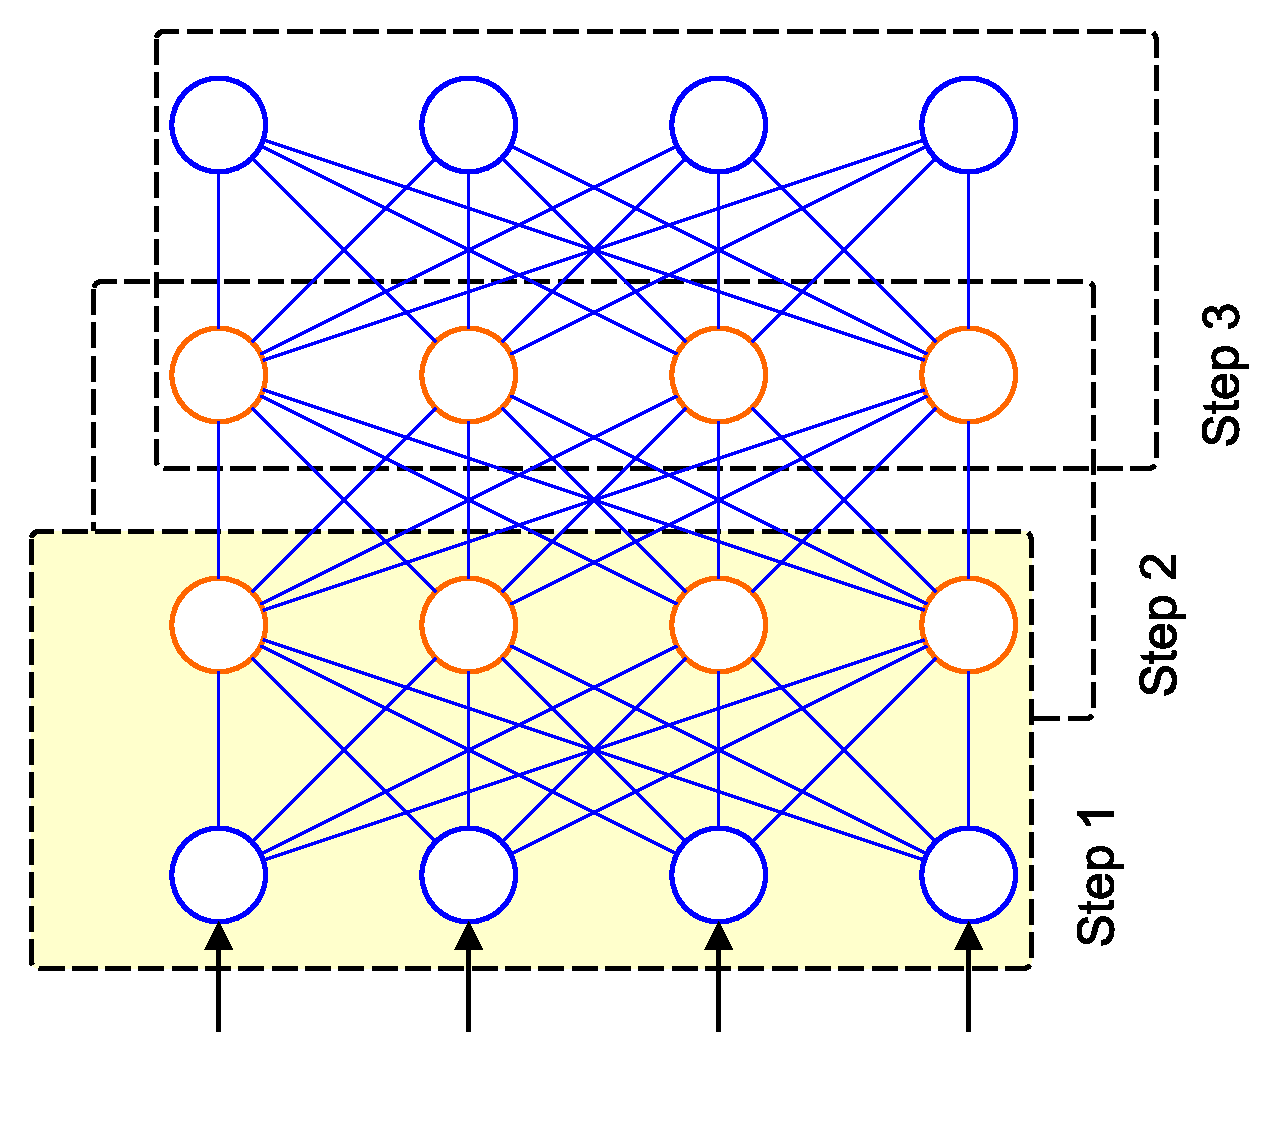
\includegraphics{dbn.pdf}}
		\end{column}
	\end{columns}

\end{frame}

\begin{frame}
	\frametitle{Outline}
	
	\begin{enumerate}
		\item Introduction
		\item Gaussian Mixture Models
		\item Convolutional Neural Networks
		\item Deep Neural Networks
		\item \textcolor{blue}{Experimental Results}
		\item Conclusions
	\end{enumerate}
\end{frame}

\begin{frame}{Experimental Results}

\begin{table}[H]
	\begin{center}
		Papers report different metrics (sentence accuracy, phone error rate) on different datasets (Bing, TIMIT) 
	\end{center}
	
	\vfill

	\centering
	\begin{tabular}{c|c|c|c|c}
		& \multicolumn{2}{c|}{Bing Mobile} & \multicolumn{2}{c}{TIMIT}\\
		Architecture & Dev. & Test  & Dev. & Test \\
		\hline
		CD-GMM-HMMM & 70.3\% & 68.4\% & & \\
		CD-DNN-HMM & 71.8\% & 69.6\% & & \\
		\hline
		CNN-HMM  & & &  & 20.07\%
	\end{tabular}

	\vfill

	\begin{center}
		Take away: Both demonstrate significant improvement over GMM approach, with CNN approach giving the best performance.
	\end{center}
\end{table}

\end{frame}

\begin{frame}
	\frametitle{Outline}
	
	\begin{enumerate}
		\item Introduction
		\item Gaussian Mixture Models
		\item Convolutional Neural Networks
		\item Deep Neural Networks
		\item Experimental Results
		\item \textcolor{blue}{Conclusions}
	\end{enumerate}
\end{frame}

\begin{frame}{Conclusions}
	\TODO{Garrett}
\end{frame}

\begin{frame}{Conclusions (Cont)}
	\TODO{Garrett}
\end{frame}

\begin{frame}
	\begin{center}
		Questions?
	\end{center}
\end{frame}

\end{document}
